\subsection{Blame Utility}
\label{sec:user-study}

%\ES{TODO: explain that we selected programs where nate got the right answer and sherrloc did NOT}

% Finally, to test the explanatory power of our blame assigments, we
% ran a user study (IRB \#2014009900) at the University of Virginia (UVA).
% %
% We included three problems in an exam in the Spring 2017 session of UVA's
% undergraduate Programming Languages course (CS 4501).
% %
% We presented the 31 students in the course with ill-typed \ocaml\
% programs and asked them to
% %
% (1) \emph{explain} the type error, and
% %
% (2) \emph{fix} the type error.
% %
% For each problem the student was given the ill-typed program and
% either \sherrloc or \toolname's blame assignment, with no error message.

We assigned three problems to the students: the |padZero| and
|mulByDigit| programs from \autoref{sec:qualitative}, as well as
the following |sepConcat| program
%
\begin{ecode}
  let rec sepConcat sep sl =
    match sl with
    | [] -> ""
    | h::t ->
        let f a x = a ^ (sep ^ x) in
        let base = (*@\hlTree{[]}@*) in
        (*@\hlSherrloc{List.fold\_left f base sl}@*)
\end{ecode}
%
where the student has erroneously returned the empty list, rather than
the empty string, in the base case of the fold.
% which triggers an error on line 7.
%
% For each problem the students were given the ill-typed program and
% either \ocaml's error or \toolname's jump-compressed trace;
%
The full user study is available in \autoref{sec:user-study-exams}.
%
Due to the nature of an in-class exam, not every student answered every
question, but we always received at least 12 (out of a possible 15 or
16) responses for each problem-tool pair.
%
%A further complication for this study is that
This session of the course
was taught in \textsc{Reason},\footnote{\url{https://reasonml.github.io}}
a dialect of \ocaml with a more C-like syntax, and thus for the study
we transcribed the programs to \textsc{Reason} syntax.

We then instructed three annotators (one of whom is an author, the others
are graduate students at UCSD) to classify the answers as
correct or incorrect.
%
We performed an inter-rater reliability (IRR) analysis to determine the
degree to which the annotators consistently graded the exams.
%
As we had more than two annotators assigning nominal (``correct'' or
``incorrect'') ratings we used Fleiss' kappa~\cite{Fleiss1971-du} to
measure IRR.\@
%
Fleiss' kappa is measured on a scale from $1$, indicating total
agreement, to $-1$, indicating total disagreement, with $0$ indicating
random agreement.

Finally, we used a one-sided Mann-Whitney $U$ test~\cite{Mann1947-fd} to
determine the significance of our results.
%
The null hypothesis was that the responses from students given
\toolname's blame were drawn from the same distribution as those
given \sherrloc's, \ie \toolname had no effect.
%
Since we used a one-sided test, the alternative to the null hypothesis
is that \toolname had a \emph{positive} effect on the responses.
%
We reject the null hypothesis in favor of the alternative if the test
produces a significance level $p < 0.05$, a standard threshold for
determining statistical significance.

\mypara{Threats to Validity}
%
Measuring understanding is difficult, and comes with its own
set of threats. % to validity.

\paragraph{Construct.}
%
We used the correctness of the student's explanation of, and fix for,
the type error as a proxy for her understanding, but it is possible
that other metrics would produce different results.
%
A further threat arises from our decision to use \textsc{Reason} syntax
rather than \ocaml.
%
\textsc{Reason} and \ocaml differ only in syntax, the type system is the
same; however, the difference in syntax may affect students'
understanding of the programs.
%
For example, \textsc{Reason} uses the notation |[h, ...t]| for the list
``cons'' constructor, in contrast to \ocaml's |h::t|.
%
It is quite possible that \textsc{Reason}'s syntax could help students
remember that |h| is a single element while |t| is a list.

\paragraph{Internal.}
%
We assigned students randomly to two groups. The first was given
\sherrloc's blame assignment for |sepConcat| and |mulByDigit|, and
\toolname's blame for |padZero|; the second was given the opposite
assignment. This ensured that each student was given \sherrloc and
\toolname problems. Students without sufficient knowledge of
\textsc{Reason} could affect the results, as could the time-constrained
nature of an exam. Thus, we excluded any answers left blank
from our analysis.

\paragraph{External.}
%
Our experiment used students in the process of learning \textsc{Reason},
and thus may not generalize to all developers. The three programs were
chosen manually, via a random selection and filtering of the programs
from the \SPRING dataset, where \toolname's top prediction was correct
but \sherrloc's was incorrect. A different selection of programs may
lead to different results.

\paragraph{Subjects.}
%
We collected exams from 31 students, though due to the nature of the
study not every student completed every problem.
%
The number of complete submissions was always at least 12 out of
a maximum of 15 or 16 per program-tool pair.
%
% While our results are not statistically significant,
% collecting more responses per test pair was not possible as it
% would require having students answer the same problem twice (once with
% \sherrloc and once with \toolname).

\begin{figure}[t]
\centering
%% EXPLAIN
\begin{tikzpicture}
\begin{axis}[
  ybar,
  % width=6cm,
  height=6cm,
  title={\large Explanation},
  ylabel={\% Correct},
  bar width=0.5cm,
  ymin=0,
  ymax=1,
  yticklabel={\pgfmathparse{\tick*100}\pgfmathprintnumber{\pgfmathresult}\,\%},
  ytick style={draw=none},
  ymajorgrids = true,
  enlarge x limits=0.25,
  symbolic x coords={{sepConcat}, {padZero}, {mulByDigit}},
  xtick=data,
  xtick style={draw=none},
  xticklabel style={align=center},
  xticklabels={
    {\texttt{sepConcat}\\($p=0.48$)},
    {\texttt{padZero}\\($p=0.097$)},
    {\texttt{mulByDigit}\\($p=0.083$)}
  },
  % x tick label style={rotate=45, anchor=north east},
  %x tick label style={font=\small},
  y tick label style={font=\small},
  reverse legend,
  transpose legend,
  legend style={legend pos = south west, font=\footnotesize},
]

% ES: NOTE: ORDER OF PLOTS/LEGEND ENTRIES MATTERS

\addplot[draw=black, fill=green2, bar shift=.25cm, error bars/.cd, y dir=both, y explicit] coordinates {
  (sepConcat, 0.8125)  +- (0, 0.0976)
  (padZero, 1.00)      +- (0, 0)
  (mulByDigit, 0.8125) +- (0, 0.0976)
};
\addlegendentry{\toolname}

\addplot[draw=black, fill=blue2, bar shift=-.25cm, error bars/.cd, y dir=both, y explicit] coordinates {
  (sepConcat, 0.80)    +- (0, 0.1033)
  (padZero, 0.875)     +- (0, 0.0827)
  (mulByDigit, 0.5714) +- (0, 0.1323)
};
\addlegendentry{\sherrloc}
\end{axis}
\end{tikzpicture}
%% FIX
\begin{tikzpicture}
\begin{axis}[
  ybar,
  % width=6cm,
  height=6cm,
  title={\large Fix},
  ylabel={\% Correct},
  bar width=0.5cm,
  ymin=0,
  ymax=1,
  yticklabel={\pgfmathparse{\tick*100}\pgfmathprintnumber{\pgfmathresult}\,\%},
  ytick style={draw=none},
  ymajorgrids = true,
  enlarge x limits=0.25,
  symbolic x coords={{sepConcat}, {padZero}, {mulByDigit}},
  xtick=data,
  xtick style={draw=none},
  xticklabel style={align=center},
  xticklabels={
    {\texttt{sepConcat}\\($p=0.57$)},
    {\texttt{padZero}\\($p=0.33$)},
    {\texttt{mulByDigit}\\($p=0.31$)}
  },
  % x tick label style={rotate=45, anchor=north east},
  %x tick label style={font=\small},
  y tick label style={font=\small},
  reverse legend,
  transpose legend,
  legend style={legend pos = south west, font=\footnotesize},
]

% ES: NOTE: ORDER OF PLOTS/LEGEND ENTRIES MATTERS

\addplot[draw=black, fill=green2, bar shift=.25cm, error bars/.cd, y dir=both, y explicit] coordinates {
  (sepConcat, 0.8125)  +- (0, 0.0976)
  (padZero, 0.9286)    +- (0, 0.0688)
  (mulByDigit, 0.7143) +- (0, 0.1207)
};
\addlegendentry{\toolname}

\addplot[draw=black, fill=blue2, bar shift=-.25cm, error bars/.cd, y dir=both, y explicit] coordinates {
  (sepConcat, 0.83)    +- (0, 0.1076)
  (padZero, 0.875)     +- (0, 0.0827)
  (mulByDigit, 0.6154) +- (0, 0.1349)
};
\addlegendentry{\sherrloc}
\end{axis}
\end{tikzpicture}
\caption[A classification of students' explanations and fixes for type
  errors, given either \sherrloc or \toolname's blame assignment.]
  {A classification of students' explanations and fixes for type
  errors, given either \sherrloc or \toolname's blame assignment.
  %
  The students given \toolname's location generally scored
  better than those given \sherrloc's.
  %
  We report the result of a one-sided Mann-Whitney $U$ test for
  statistical significance in parentheses.}
\label{fig:user-study-results}
\end{figure}


% \begin{figure}[t]
% \centering
% % \centerline{
% % \begin{minipage}{1.2\textwidth}
% % \centering
% 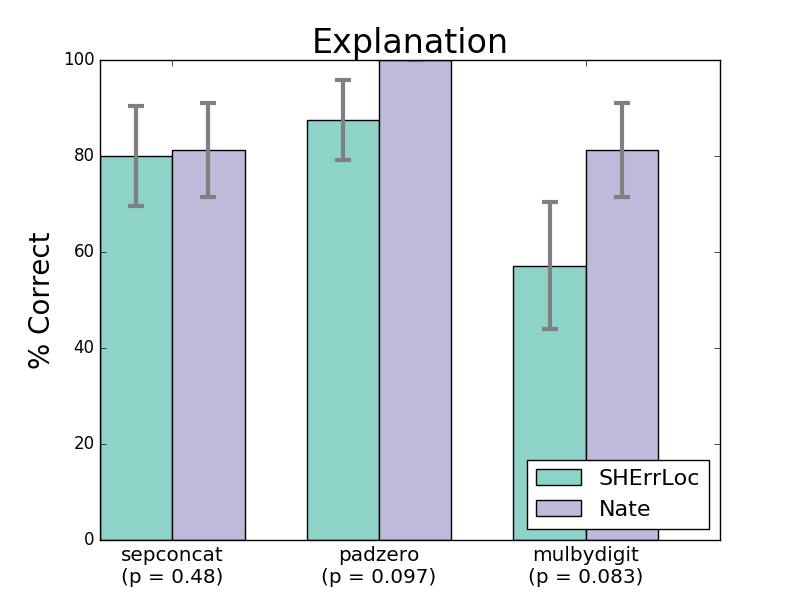
\includegraphics[width=0.49\linewidth]{user-study-reason.png}
% 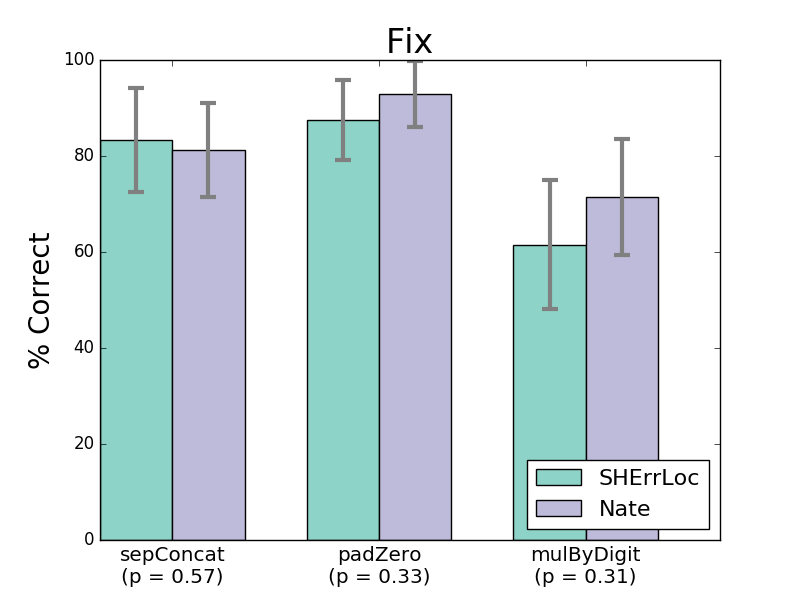
\includegraphics[width=0.49\linewidth]{user-study-fix.png}
% % \end{minipage}
% % }
% % \vspace{3ex}
% \caption[A classification of students' explanations and fixes for type
%   errors, given either \sherrloc or \toolname's blame assignment.]
%   {A classification of students' explanations and fixes for type
%   errors, given either \sherrloc or \toolname's blame assignment.
%   %
%   The students given \toolname's location generally scored
%   better than those given \sherrloc's.
%   %
%   We report the result of a one-sided Mann-Whitney $U$ test for
%   statistical significance in parentheses.}
% \label{fig:results-user-study}
% \end{figure}

\mypara{Results}
%
The measured kappa values were $\kappa = 0.68$ for the explanations and
$\kappa = 0.77$ for the fixes; while there is no formal notion for what
consititutes strong agreement~\cite{Krippendorff2012-wd}, kappa values
above $0.60$ are often called ``substantial''
agreement~\cite{Landis1977-ey}.
%
Figure~\ref{fig:results-user-study} summarizes a single annotator's
results, which show that students given \toolname's blame assignment
were generally more likely to correctly explain and fix the type error
than those given \sherrloc's.
%
There was no discernible difference between \toolname and
\sherrloc for |sepConcat|; however, \toolname responses for |padZero| and
|mulByDigit| were marked correct 5--25\% more often than the \sherrloc
responses.
%
While the results appear to show a trend in favor of \toolname,
they do not rise to the level of statistical significance;
further investigation is merited.
% The results appear to show a trend in favor of \toolname;
% %
% however, none rise to the level of statistical significance.
%
